\begin{figure}[H]
  \centering
  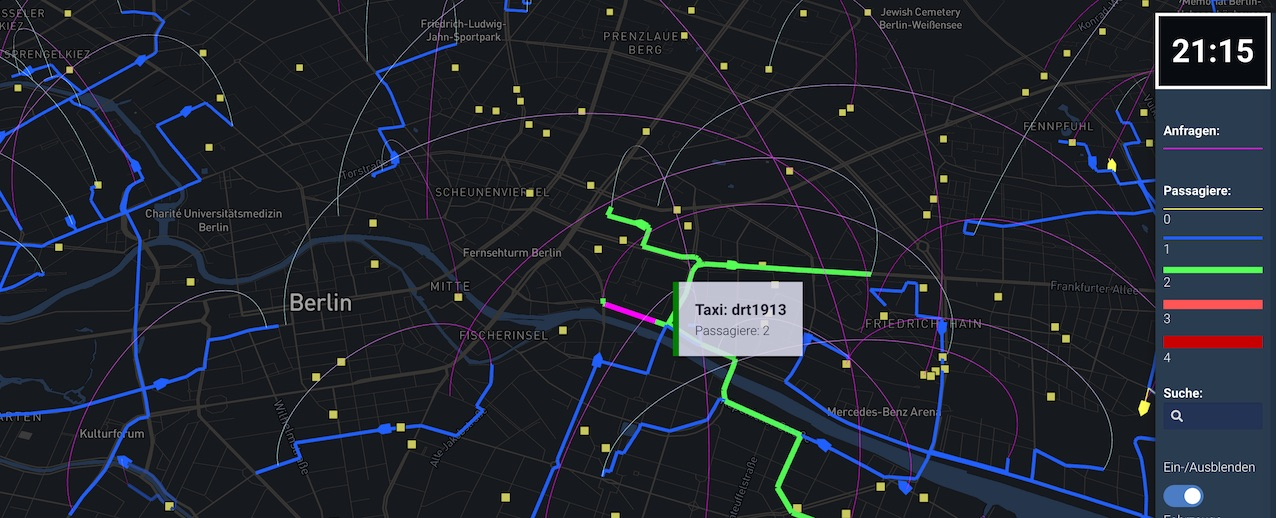
\includegraphics[width=0.8\textwidth]{assets/drt.jpg}
  \caption{Animation of DRT vehicle, paths, and passenger requests}
\end{figure}

\hypertarget{usage}{%
\subsection{Usage}}

A file named \texttt{viz-vehicle-*.yml} must be present in working
folder. Each yml file matching that pattern will produce a separate DRT
visualization.

\textbf{drt-example.yml}

\begin{lstlisting}
  title: 'Dynamic Response Shared Taxis'
  description: Inactive Sammeltaxis (Quadrat); Aktive Sammeltaxis (yellow)
  drtTrips: drt-vehicles.json.gz
  thumbnail: thumbnail-vehicles.jpg
  center: [13.391, 52.515]
\end{lstlisting}

\hypertarget{yaml-fields-explained}{%
\subsection{YAML fields explained}\label{yaml-fields-explained}}

\noindent\textbf{drtTrips:} the output from the
\href{https://github.com/simwrapper/simwrapper/raw/master/scripts/parse-drt-link-events.py}{parse-drt-link-events.py}
script, gzipped for best performance

\noindent\textbf{center:} Use this to force the map center point.
\texttt{{[}long,lat{]}}
